\section{Visualizations}
We propose three interactive visualizations by first analysing a set of tasks our application should solve~(cf. Section~\ref{tasks}), and then deriving specific requirements for the included visualizations~(cf. Section~\ref{requirements}). Furhtermore, we discus expressiveness, effectiveness, and appropriateness for each of the three implemented visualizations~(cf. Section~\ref{presentation}) and explain the interactivity of the visualization application~(cf. Section~\ref{interaction}).

\subsection{Analysis of Application Tasks}
\label{tasks}
\begin{table}
    \caption{Exemplary questions that should be answered by visualizions of French road accident dataset, with the typical background a person asking that question would likely have.}
    \label{table-questions}
    \begin{tabularx}{\linewidth}{cXp{0.3\linewidth}}
        \toprule
        \textbf{\#} & \textbf{Question} & \textbf{Background} \\
        \midrule
        1 & Are roads more dangerous in winter or summer? & citizen \\
        2 & Do older or younger people drive more safely? & policy maker \\
        3 & Are there hotspots of accidents in cities or rural areas? & citizen, policy maker \\
        4 & If hotspots occur, which other characteristics can explain the correlations. & policy maker \\
        5 & Do the proportion of dead and injured persons correlate? & policy maker \\
        6 & Where are unproportionately more people killed in traffic? & policy maker \\
        7 & Do dedicated bicycle lanes make roads safer for cyclists? & citizen, policy maker, infrastructure planner \\
        8 & Are wider roads safer than narrow roads? & citizen, infrastructure planner \\
        \bottomrule
    \end{tabularx}
\end{table}
Because of the diverse application background and target groups described in Section~\ref{introduction}, many tasks can be formulated to be answered by data visualizations. To narrow down the tasks, in this report, we propose a set of exemplary questions our visualizations should answer. The questions listed in Table~\ref{table-questions} also specify the most likely background a person asking that question would have. This additional context allows us to fine-tune individual visualizations by assuming background knowledge from the respective target group.
We identify 3~mental models as most important to help people answer the abovementioned questions: \Ni times and dates, \Nii geographical position, \Niii clustering or categorization.
Time and date, for example, are important to identify periodical trends, as required in question~1 in Table~\ref{table-questions}. A time series plot is able to capture the continuity of time and express a single data dimension in relation to time, which is enough for identifying the dangerousness of specific time periods.
Geographical position is crucial for understanding local patterns, as required in questions~3 or~6. While most people are very familiar with using maps as visualization for geographically positioned data, it is often not obvious how to visualize the multiple dimensions of the data points that are displayed on that map. We argue that given the space constraints of a map, the stick figures technique~\cite{PickettG1988} is appropriate because it can display a fixed number of dimensions in small space while observers can still detect patterns across the maps geographical dimensions.
And clustering accident occasions with respect to different categories is needed for comparing how different characteristics might influence road safety, as required in question~7. When working with multidimensional data, like we do with accidents, trees and treemaps~\cite{Shneiderman1992} can be a good visualization to present different, hierarchical categories.

\subsection{Visualization Requirements}
\label{requirements}
We derive 3~main goals that our visualization application should implement: \Ni to identify dangerous regions, times, and situations, \Nii to summarize trends with respect to time and location, and \Niii to offer detailed views where data is aggregated.
Identifying dangerous patterns should be supported by emphasizing road injuries or road deaths at first glance or by showing differences of accidents' characteristics with respect to visual reference points.
Accidents that follow a specific pattern should be distinguishable from other accidents.
Time-based trends should be made visible both in the long term and in the short term. Geographical trends must also include the geographical position but should not over-emphasize it to be effective.
And to avoid losing important details such as outliers, the visualizations should always feature a way to show the data with as little aggregation~(e.g., average, minimum, maximum) as possible, while still not overwhelming observers of the visualization.

\subsection{Visualization Presentation}
\label{presentation}
The visualization application proposed to solve the aforementioned tasks~(cf. Section~\ref{tasks}) consists of three interatively combined visualization pages: \Ni a time series plot to compare the number of accidents or casualties, \Nii a geographical map of icon-based stick figure visualizations, and \Niii a treemap view of hierarchically categorized accidents.

\subsubsection{Severity Time Series}
\begin{figure}
    \centering
    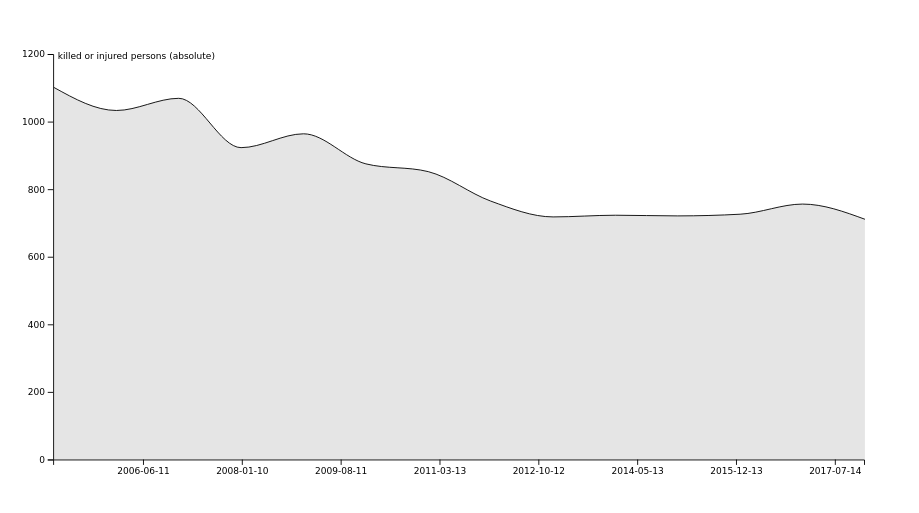
\includegraphics[width=0.9\linewidth]{figures/time-series-2-to-1-killed-or-injured-absolute-never-per-year.png}
    \caption{Time series of the number of killed or injured persons per year from~2005 to~2020 with a 2:1~aspect ratio.}
    \label{figure-time-series-killed-injured-per-year}
\end{figure}
\begin{figure}
    \centering
    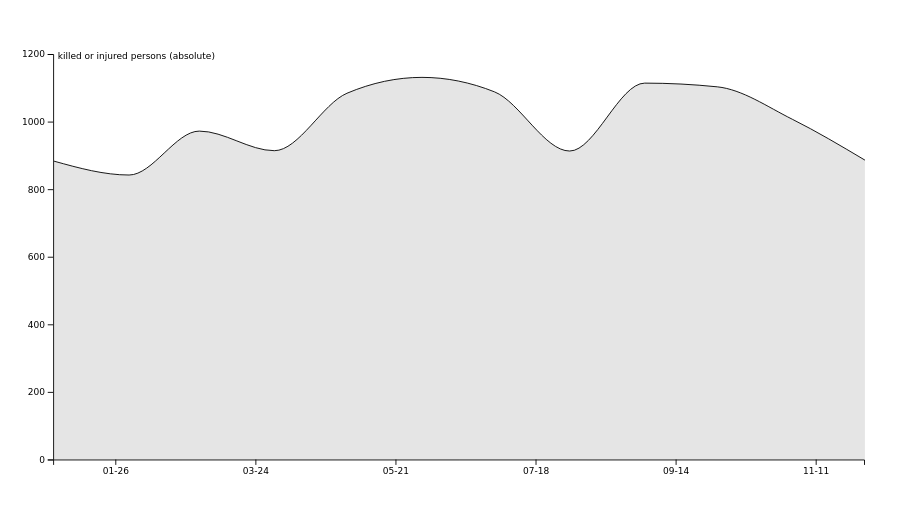
\includegraphics[width=0.9\linewidth]{figures/time-series-2-to-1-killed-or-injured-absolute-by-year-per-month.png}
    \caption{Time series of the number of killed or injured persons per month with a 2:1~aspect ratio, by aggregating across all years~2005--2010.}
    \label{figure-time-series-killed-injured-by-year-per-month}
\end{figure}
\begin{figure}
    \centering
    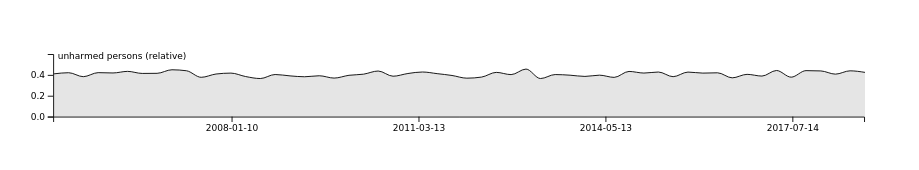
\includegraphics[width=0.9\linewidth]{figures/time-series-banking-45-unharmed-relative-never-per-quarter.png}
    \caption{Time series of the proportion of unharmed persons of all persons involved in accidents per quarter with banking to~45\(^\circ\).}
    \label{figure-time-series-banking-unharmed-relative-per-quarter}
\end{figure}
The first visualization we introduce is a time series plot of the prevalence and severity of accidents across time.
Users can optionally choose to aggregate accidents across years~(to find seasonal patterns) and can count the number of persons per week, month, or year. They can also choose whether killed, injured, killed and injured, unharmed, or all persons should be counted. Additionally one can choose to display the absolute number or relative proportion of persons that fit the above criteria, and adjust the plot's aspect ratio.
Figures~\ref{figure-time-series-killed-injured-per-year}, \ref{figure-time-series-killed-injured-by-year-per-month}, and~\ref{figure-time-series-banking-unharmed-relative-per-quarter} illustrate this visualization.
To support users in distinguishing different slopes in the plot, we allow users to automatically compute the optimal aspect ratio by banking to~45\(^\circ\).
As the number or proportion of persons is quantitative data, it is visually the easiest to map the data to a position, in this case the height of the plotted line. It is also easy for humans to distinguish slopes in lines. This way in the time series line users can, for example, easily spot periods where the number of injured persons increases, decreases, or stagnates.
When users choose to aggregate the accidents across all years, it would also seem intuitive to visualize that periodical data in a radial plot. However, in such plot the slope differences are more difficult to spot, limiting that approach's expressiveness. The recursive pattern technique is also a good choice for periodical data, but we argue that the difficulty of mapping a color to quantitative data, as would be the case with a recursive pattern visualization, is cognitively more difficult than mapping from a position, making the visualization more effective but less expressive. Therefore, we choose a line plot in the cartographic coordinate system.

\subsubsection{Geographical Map with Person Characteristics Stick Figures}
\begin{figure}
    \centering
    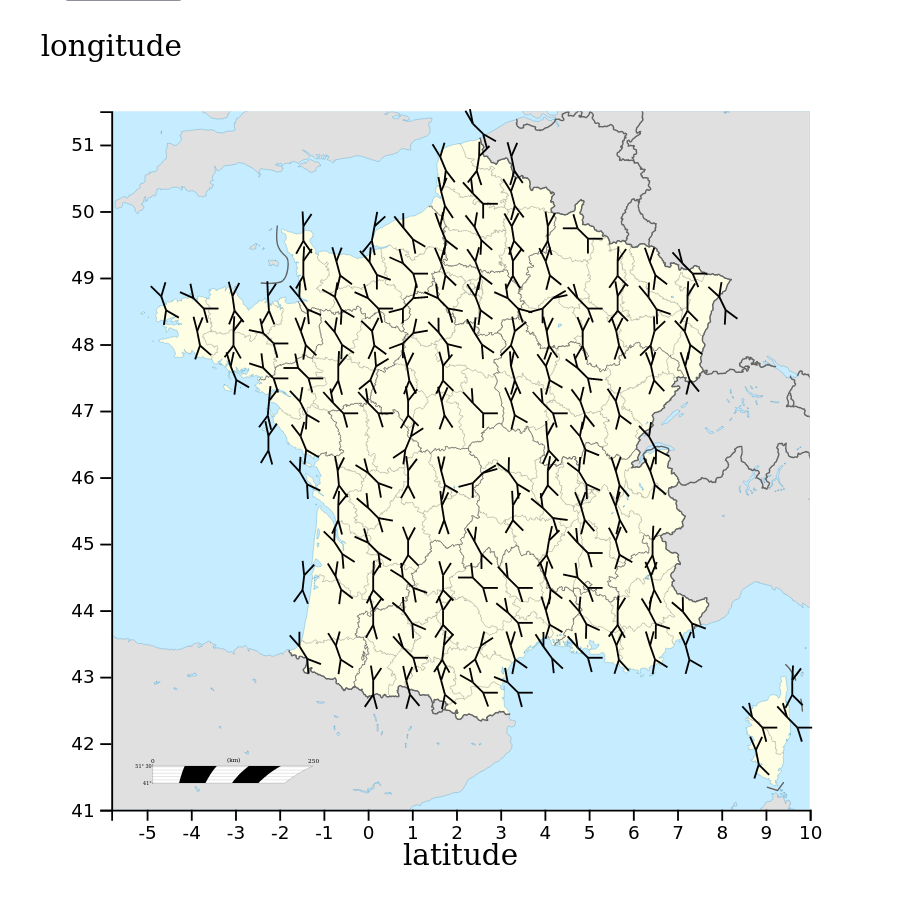
\includegraphics[width=0.6\linewidth]{figures/stick-figures-by-grid-20-20-average.png}
    \caption{Stick figure icons of average person characteristics on a map of France after partitioning the map into a \(20 \times 20\)~grid.}
    \label{figure-stick-figures-grid-average}
\end{figure}
\begin{figure}
    \centering
    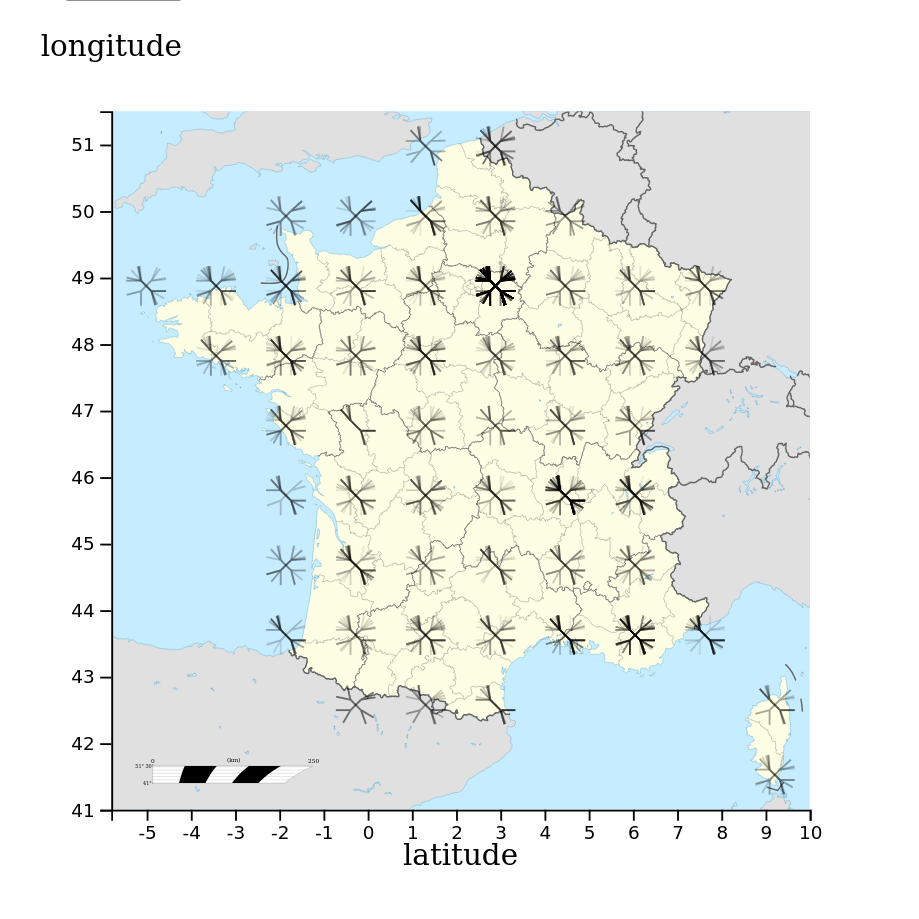
\includegraphics[width=0.6\linewidth]{figures/stick-figures-by-grid-10-10-xray.png}
    \caption{Stick figure icons of person characteristics on a map of France after partitioning the map into a \(10 \times 10\)~grid. Each group's stick figures are overlayed in x-ray style.}
    \label{figure-stick-figures-grid-xray}
\end{figure}
\begin{figure}
    \centering
    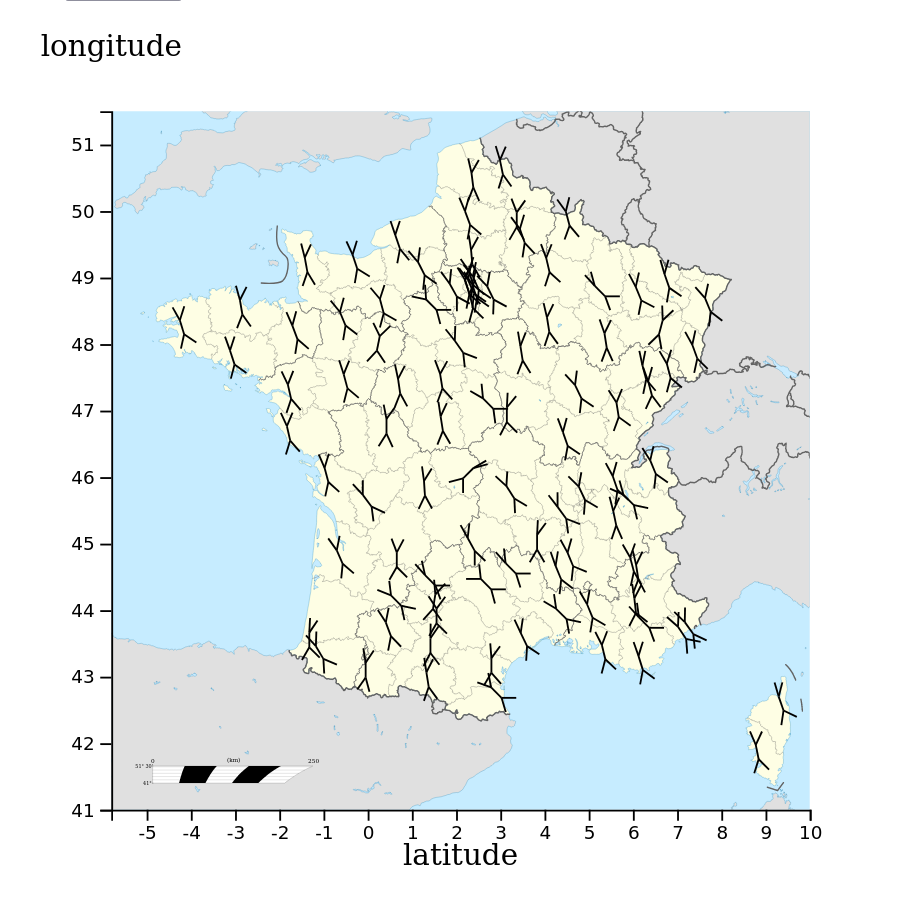
\includegraphics[width=0.6\linewidth]{figures/stick-figures-by-department-average.png}
    \caption{Stick figure icons of average person characteristics on a map of France after partitioning the map into France's official Departements.}
    \label{figure-stick-figures-departments-average}
\end{figure}
To visualize geographical characteristics of involved persons, we display stick figure icons~\cite{PickettG1988} of aggregated person groups on an equirectanguular geographical map projection of France\footnote{\url{https://commons.wikimedia.org/wiki/File:France_location_map-Regions_and_departements-2016.svg}}.
Users can either choose to display one single stick figure per group, visualizing the average values of that group, or to display each instance within a group as a separate stick figure, following the x-ray design pattern.
Figures~\ref{figure-stick-figures-grid-average}, \ref{figure-stick-figures-grid-xray}, and~\ref{figure-stick-figures-departments-average} illustrate this visualization.
In this second visualization, the dominating mental model is geographical position, which is commonly associated with maps. Hence, we map the geographical position to coordinates on the map. As we want users to quickly spot patterns in the displayed data, i.e., differences across regions of the map, textures are a good visualizions technique.
By plotting stick figures on a grid of the map, such a texture can emerge. We map the following 5~characteristics to the 5~angles of each stick figure:
\begin{description}
    \setlength{\itemsep}{1pt}
    \item[\(\alpha\)] sex, either \(-45^\circ\)~(female) or \(45^\circ\)~(male)
    \item[\(\beta\)] birth year, inverted, mapped to  \([105^\circ; 135^\circ]\)
    \item[\(\gamma\)] travel reason, ordered~(professional, home\(\to\)work, home\(\to\)school, shopping, walking/leisure), mapped to  \([105^\circ; 135^\circ]\)
    \item[\(\delta\)] safety equipment count, inverted, mapped to  \([105^\circ; 135^\circ]\)
    \item[\(\epsilon\)] number of persons in vehile, inverted, mapped to  \([105^\circ; 135^\circ]\)
\end{description}
Mapping the nominal dimension of the person's sex to the stick figure's angle makes it particularly easy to spot differences between female and male drivers. For example, in Figure~\ref{figure-stick-figures-grid-average} one can clearly identify that the average person involved in an accident is male.
Apart from other icon-based visualization techniques which we did not use due to the large number of data points~(e.g., Chernoff faces~\cite{Chernoff1973}---otherwise more expressive---would clutter the available space on the map too much, making it more difficult to distinguish individual icons), we also discourage heatmaps for this dataset, because they can only visualize one dimension other than the geoposition and would suffer from issues when decoding ordinal values from their color.
We argue that therefore stick figure icons are the most effective technique to visualize multi-dimensional characteristics of persons involved in accidents.
To fulfil the third visualizaiton requirement, not hiding details behind averages, each person involved in an accident can also be shown as an individual stick figure. Here we make the stick figure translucent so that multiple stick figures can be overlayed and produce a density plot as is commonly used in parallel coordinates plots~\cite{Wegman1990}.
This technique still allows for visualizing trends but, for example, we can now distinguish characteristics of female and male persons, where the sex information would otherwise be lost in aggregation by average.

\subsubsection{Accident Type Treemap}
\begin{figure}
    \centering
    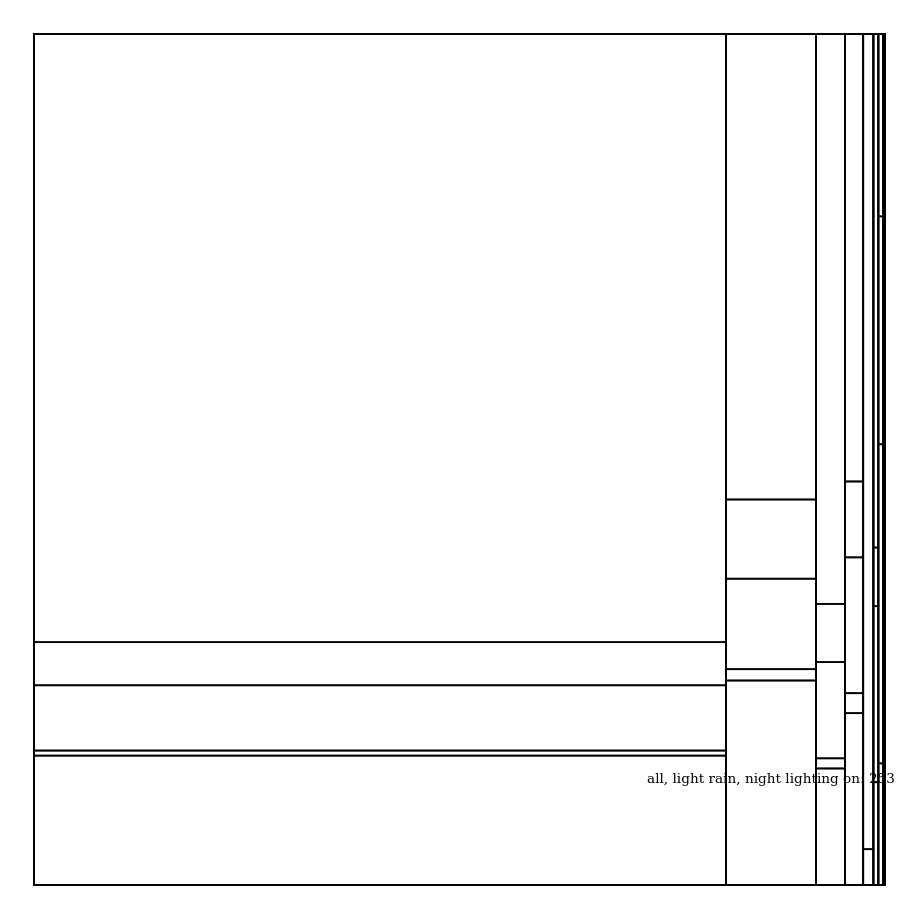
\includegraphics[width=0.6\linewidth]{figures/tree-treemap-weather-light-condition.png}
    \caption{Tree map of accidents by weather and light condition.}
    \label{figure-treemap-weather-light-condition}
\end{figure}
\begin{figure}
    \centering
    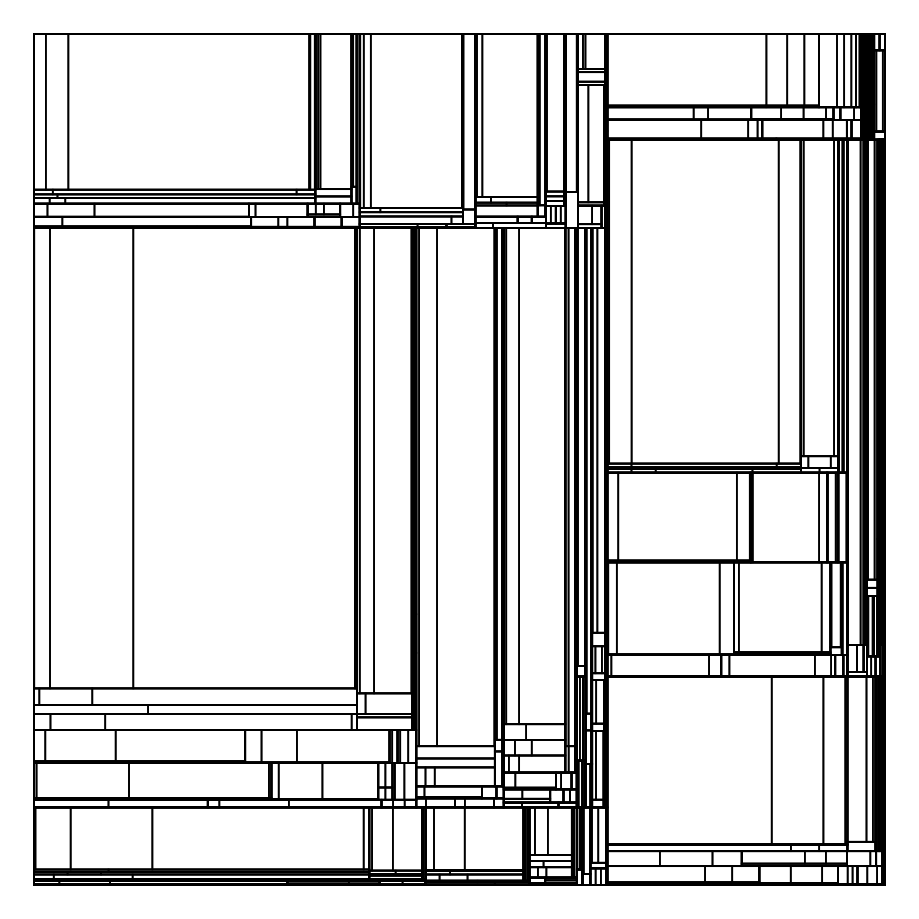
\includegraphics[width=0.6\linewidth]{figures/tree-treemap-location-type-traffic-regime-intersection-type-road-curvature-road-profile-dedicated-line-road-category.png}
    \caption{Tree map of accidents by location type, traffic regime, intersection type, road curvature, road profile, dedicated lines, and road category.}
    \label{figure-treemap-many}
\end{figure}
Our third visualizaiton focuses on the task of identifying categories in which road accidents most often happen. We implement this task by first clustering the accident dataset hierarchically by multiple categorical dimensions where the number of accidents that fall into each set of categories represents a weight. The resulting weighted tree can then be displayed in three different ways: \Ni as a nested list, \Nii as a graph, and \Niii as a treemap~\cite{Shneiderman1992}.
Users can also reorder the dimensions across which the tree is partitioned, and they can enable or disable partitioning for specific dimensions.
Figures~\ref{figure-treemap-weather-light-condition} and~\ref{figure-treemap-many} illustrate the treemap visualization.
Because the dataset contains many nominal dimensions~(cf. Section~\ref{data}) visually mapping accidents to length or angles would make the visualization less effective. Instead, for nominal data mapping to areas where similar areas are close together is more effective.
In the graph view this mental connection is supported by connecting the graph's nodes with a line. On a treemap, this connection is achieved by placing the rectangles of child categories inside the rectangle of their parent category, satisfying the mapping methodology of surrounding.
It is easier for users to read an individual category's description in the graph and list views. By showing category names of node in the treemap when a user hovers their mouse cursor above the corresponding rectangle, we circumvent this limitation.
Nonetheless, we keep the list and graph visualizations to allow users to traverse the tree's hierarchy more effectively, once they have found a category of interest.
The treemap visualization also gives an intuitive way to identify majority categories of accidents because viewers can easily spot the largest rectangles of the treemap even in cluttered treemaps as illustrated in Figure~\ref{figure-treemap-many}. The rectangle's size effectively expresses the number of accidents.

\subsection{Interaction}
\label{interaction}
One of the requirements we formulated~(cf. Section~\ref{requirements}) is to be able to explore details. 
We see an interaction between the three proposed visualizations as an oportunity to fulfil that goal and to encourage viewers to explore differences for groups of similar accidents~(both in terms of geographical region as well as for characteristics).
Therefore viewers are given the option to select filtered subsets of the accidents to explore them in a different visualization.
This filtering is possible in two places: \Ni by selecting geographical clusters from the stick figure visualization map and \Nii by selecting nodes from the tree visualized in the accident characteristics treemap.
The first case is especially useful for citizens who want to focus their exploration on just their home town~(shown in Figure~\todo{example screenshot}). They can then, for example, switch to the severity time series to find out when to avoid driving specifically in their home town or find out what the most common accident types are by switching to the tree visualization. The second case is most useful for policy makers or public infrastructure planners because they can first identify a target problem they want to mitigate in the treemap visualization. Then they could, for example, explore where that type of accident occurs most often~(e.g., to plan an infrastructure project, as exemplified in Figure~\todo{example screenshot}) or what persons are often involved~(e.g., to educate or regulate that group of persons). Filtering by local characteristics such as road curvature or slopes can also be useful for identifying periodical patterns with the time series visualization, for example to apply measures only in summer or winter.
As the three visualizations are already complex and feature high-dimensional data, we refrain from embedding individual visualizations into others as pop-up.
We also planned to implement a time range selector to filter accidents by time or season, but had to omit that filter due to the time constraints.
